% !TEX root = main.tex
\documentclass{article}
\usepackage{../include/report_style}

\title{Project Proposal}
\author{Juan Carlos Cruz - ira406}
\date{ME 5703 Lean Product Development and Service Systems}

\begin{document}
	\maketitle
	\noindent%

	% Introduction
	\section{Introduction}

	The Department of Defense (DoD), which includes the U.S. Army, Navy, Air Force, Marine Corps, Space Force, National Security Agency, Defense Intelligence Agency, National Geospatial-Intelligence Agency, and National Reconnaissance Office, is traditionally viewed as a bureaucratic and slow-moving organization due to its sheer size and complexity.

	For my research proposal, I aim to investigate the implementation of lean and six-sigma principles within the DoD and its affiliated organizations to identify if these principles have been successful in improving the efficiency and effectiveness of the DoD.
	To better understand research trends regarding lean and six-sigma implementation regarding the DoD, a scientometric review is conducted.
	Following the procedure outlined in \cite{MA2023104828}, the review begins by selecting an appropriate database, tailoring a search term criteria, filtering the results, and then analyzing the key research themes appearing across the resulting works.

	The complete citation dataset, analysis code, and figures can be found at \url{https://github.com/jc-cr/lean_dod_paper}.

	% Analysis setup

	\section{Scientometric Setup}

	ProQuest was selected as the primary database for this search as it yielded the most results, 481 total, including Theses, Trade journals, Scholarly Articles, and Conference Papers.

	The author also reviewed the Web of Science, Lens, and the Defense Technical Information Center, but found these to have insufficient paper results for this analysis.

	One downside to this search method is that valuable "Grey literature" including government web articles and reports are not included within the analysis, this limitation will be covered in the final report by including such literature in the final review.

	The search term used in ProQuest was as follows:

	\begin{minipage}{\linewidth}
	\begin{spacing}{0.8}
	\noindent\texttt{AB("Department of Defense" OR "DoD" OR "DOD" OR "U.S. Army" OR} \\
	\texttt{"Department of the Army" OR "U.S. Navy" OR "Department of the Navy" OR} \\
	\texttt{"U.S. Air Force" OR "Department of the Air Force" OR "U.S. Marine Corps" OR} \\
	\texttt{"U.S. Space Force" OR "National Security Agency" OR "NSA" OR} \\
	\texttt{"Defense Intelligence Agency" OR "DIA" OR "National Geospatial-Intelligence} \\
	\texttt{Agency" OR "NGA" OR "National Reconnaissance Office" OR "NRO")} \\
	\texttt{AND FT("six sigma" OR "6$\sigma$" OR "lean six sigma" OR} \\
	\texttt{"continuous process improvement" OR "LSS") AND LA(EN)}
	\end{spacing}
	\end{minipage}


	The resulting papers were inspected and cleaned manually for irrelevant documents or duplicates, leaving 465 documents to analyze.
	The results were exported to a xlsx file and then analyzed with a python script.

	The python analysis program was setup to output graphs related to the following items:

	\begin{itemize}
		\item \textbf{Publication Trend Analysis}: Temporal distribution of publications by year, including trend lines and 3-year moving averages to identify patterns in research activity.
		
		\item \textbf{Document Type Classification}: Analysis of publication types (e.g., journal articles, case studies, dissertations).
		
		\item \textbf{Keyword Analysis}: Extraction and frequency analysis of keywords from abstracts, including removal of common stopwords and use of lemmatization for term normalization.
		
		\item \textbf{Network Analysis}: Construction of keyword co-occurrence networks to visualize relationships between concepts in the literature, with filtering to highlight the most significant connections.
		
		\item \textbf{Topic Modeling}: Latent Dirichlet Allocation (LDA) modeling to identify underlying thematic structures across the corpus of abstracts.
		
		\item \textbf{Thematic Trend Analysis}: From prior analysis, analysis of the identified themes in the literature over time.

		\item \textbf{Thematic Distribution}: Distribution of themes across the corpus of abstracts.
	\end{itemize}

	The results and figures generated from these analysis methods are presented in the following sections.

	\section{Scientometric Analysis}

	As seen in \figref{fig:publication_trend}, from the earliest publications found in 1992 up to 2025, there has been an increasing trend for lean six sigma related publication related to the DoD and it's affiliated organizations.
	The year 2017 saw the most amount of publication related to lean six sigma and the DoD.
	Interestingly, since 2017 there has been a downward trend in lean six sigma literature.


	\begin{figure}[htbp]
	\centering
	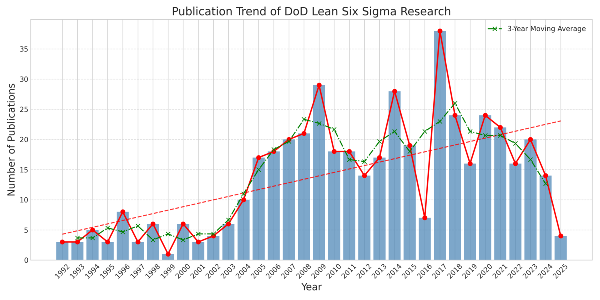
\includegraphics[width=0.9\linewidth,height=0.9\textheight,keepaspectratio]{publication_trend}
	\caption{Publications in lean six sigma from database search}
	\label{fig:publication_trend}
	\end{figure}

	The majority of the publication types found in the ProQuest database are Dissertation/Thesis, with Feature, and General Information documents following after.
	This is visualized in \figref{fig:document_type}
	The trends over time for the different document classes is shown in \figref{fig:document_type_trend}.

	\begin{figure}[htbp]
		\centering
		\begin{subfigure}[b]{0.48\textwidth}
			\centering
			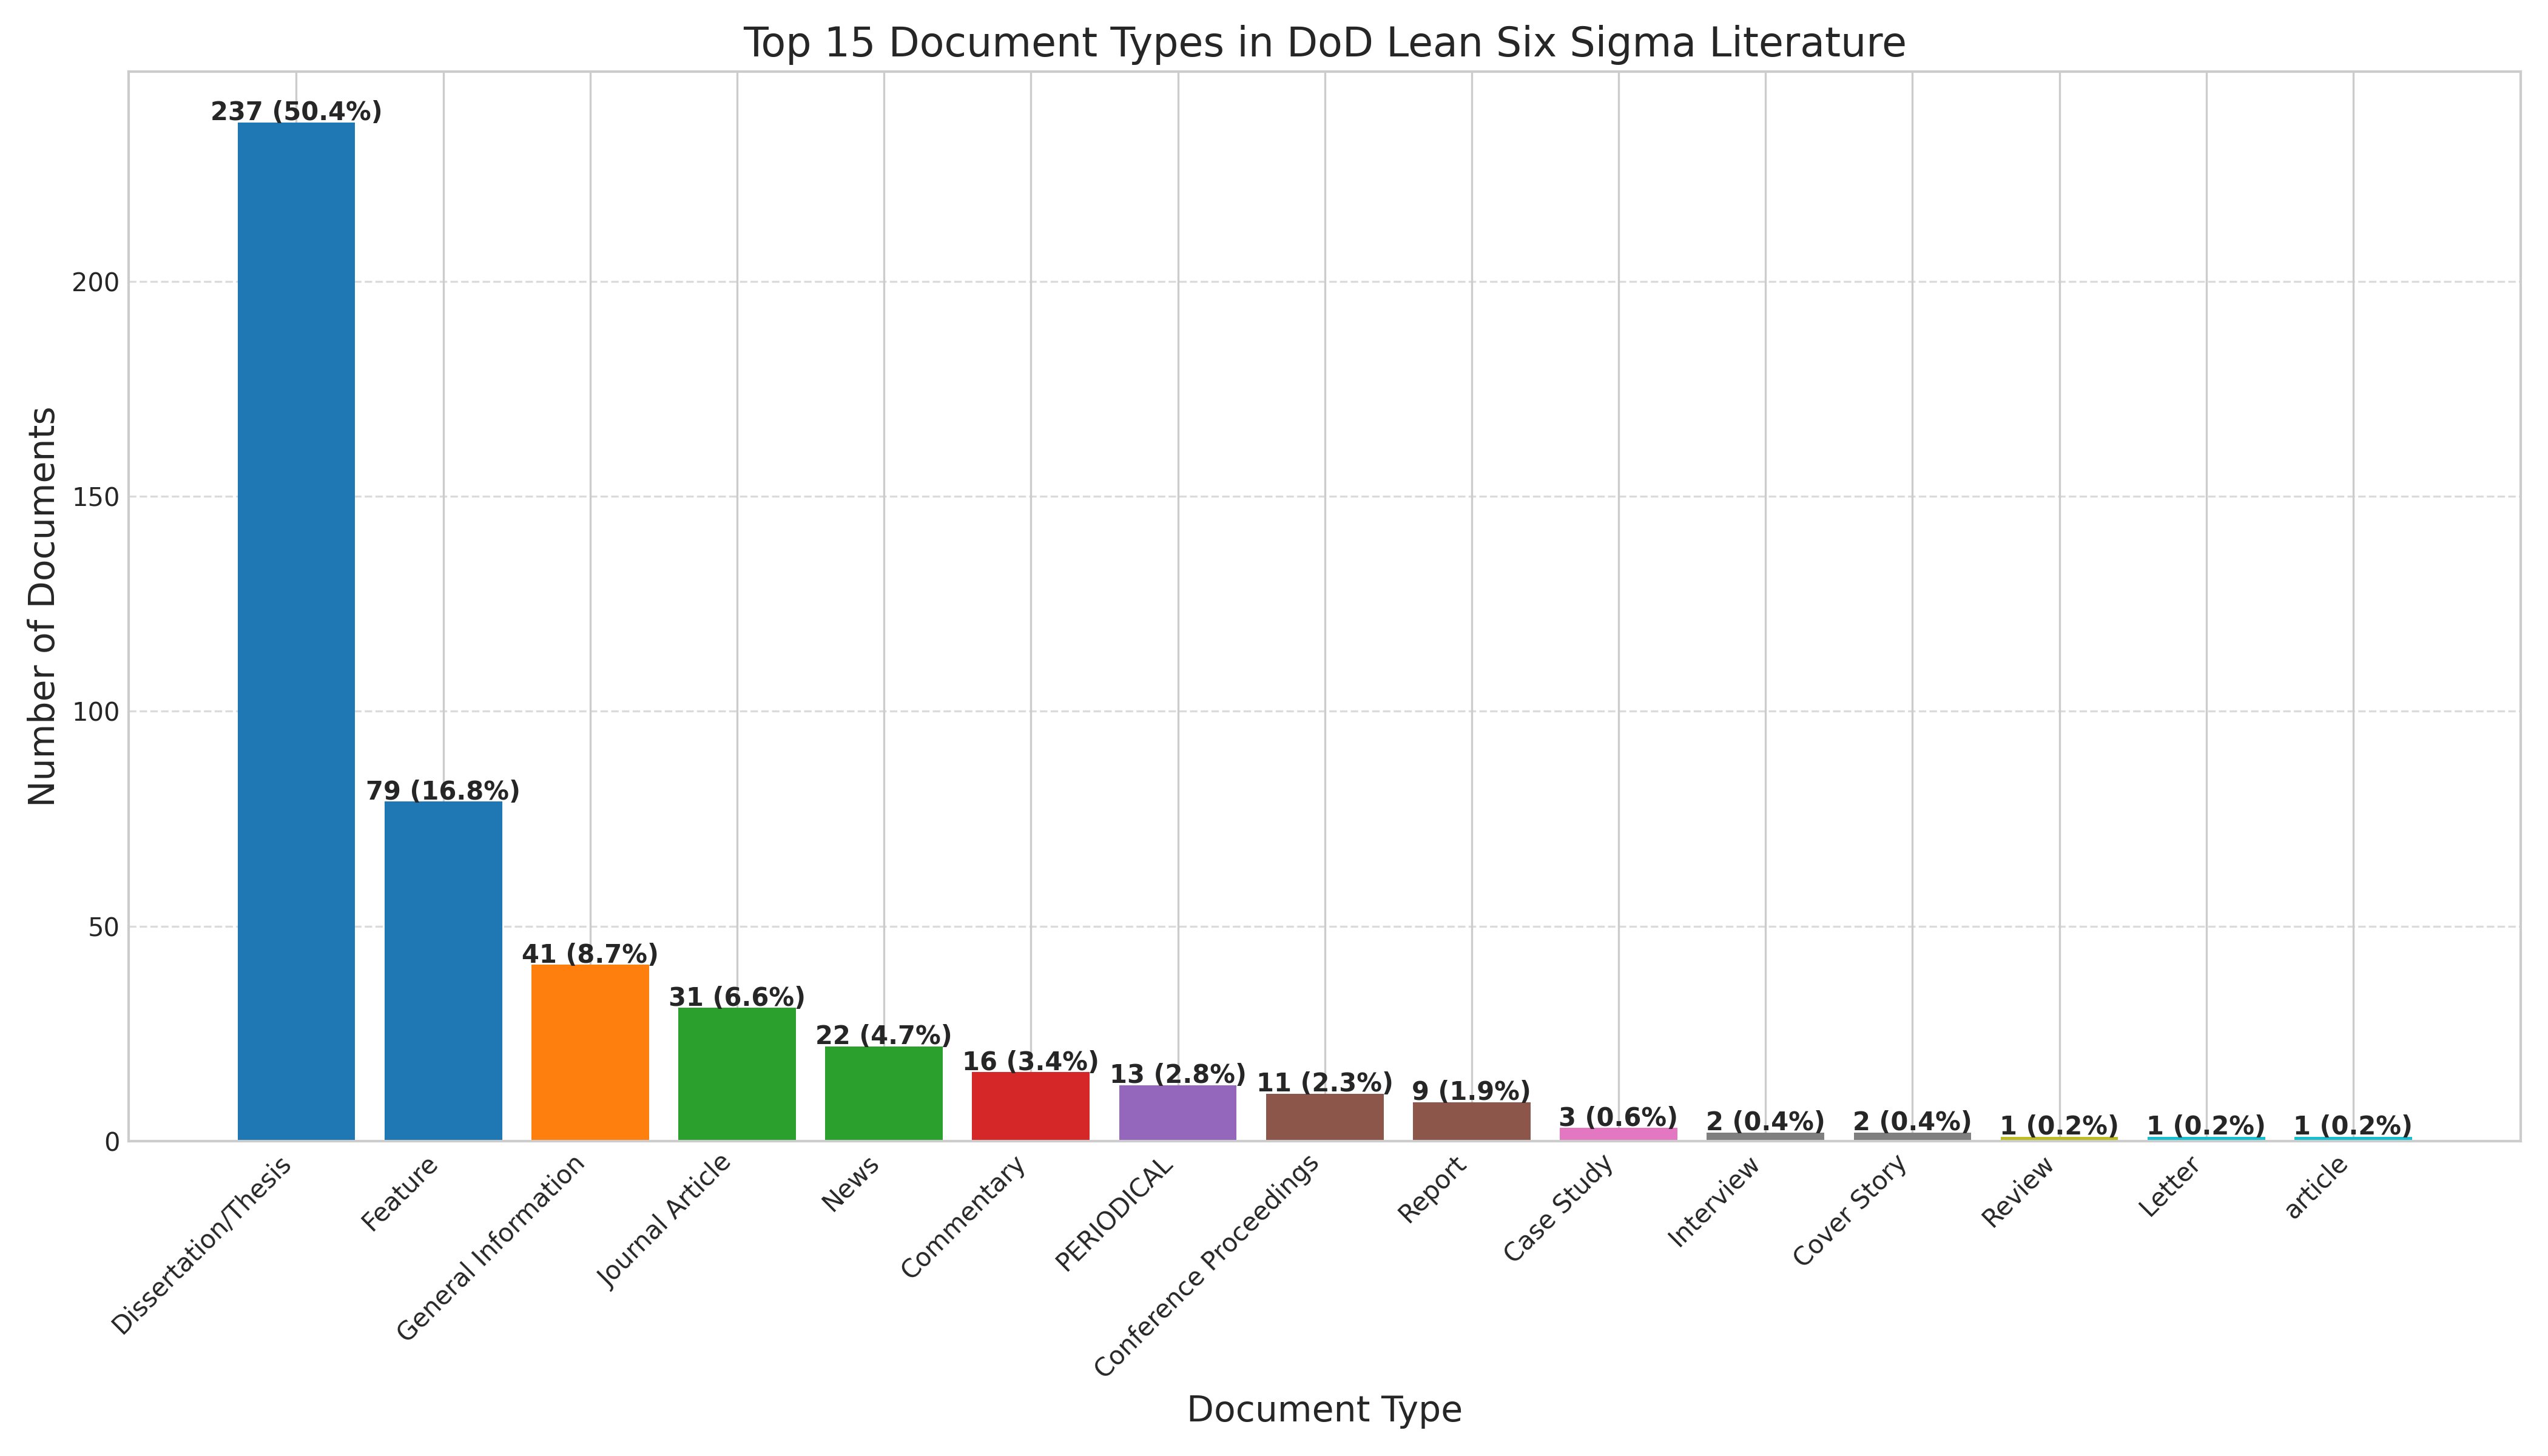
\includegraphics[width=\textwidth,height=0.35\textheight,keepaspectratio]{document_type_distribution_bar}
			\caption{Types of publications found in the database search}
			\label{fig:document_type}
		\end{subfigure}
		\hfill
		\begin{subfigure}[b]{0.48\textwidth}
			\centering
			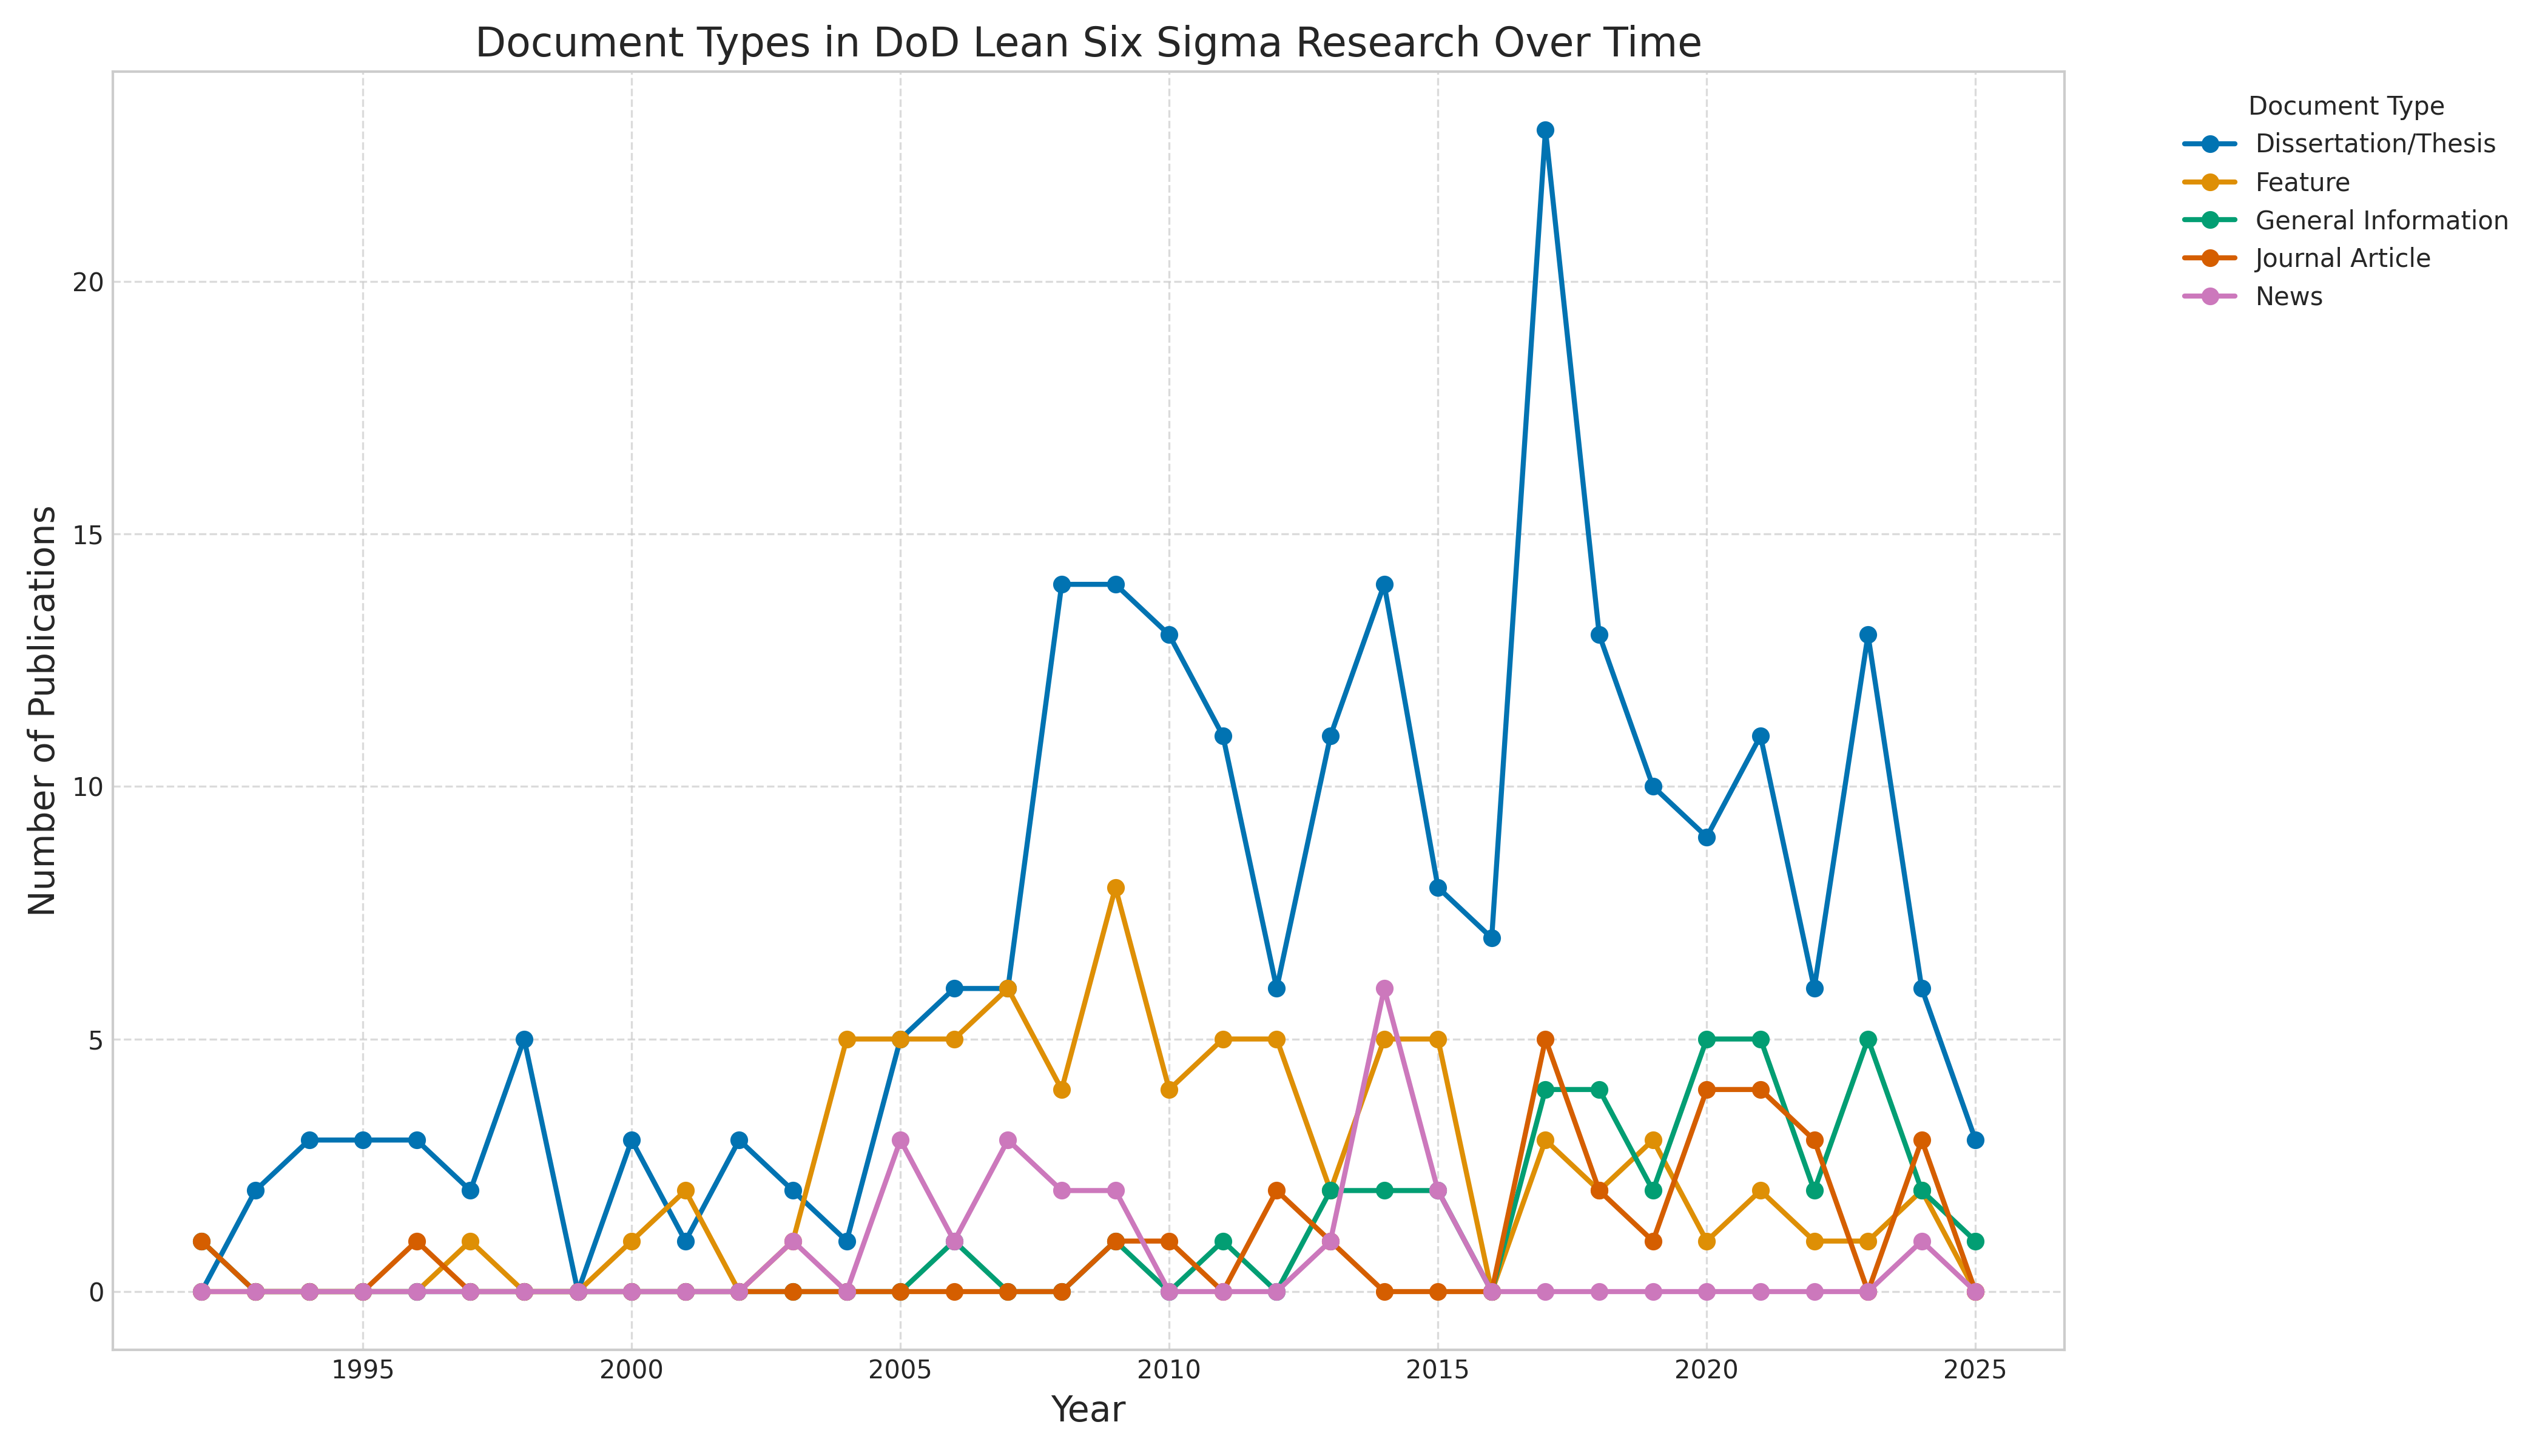
\includegraphics[width=\textwidth,height=0.35\textheight,keepaspectratio]{document_type_trends}
			\caption{Trend over time for the different document types}
			\label{fig:document_type_trend}
		\end{subfigure}
		\caption{Analysis of document types and their trends over time}
		\label{fig:document_analysis}
	\end{figure}


	Analyzing the keywords present in the document abstracts, \figref{fig:keyword_freq} shows that \textit{system}, \textit{process}, and \textit{management} appear with the highest frequency across all documents.

	From the co-occurrence network in \figref{fig:keyword_network}, we observe that \textit{management}, \textit{data}, and \textit{process} have a high betweenness centrality, indicating they serve as important bridges connecting other keywords in the literature. This suggests these concepts play central roles in linking different aspects of lean six sigma implementation within DoD contexts.

	A Latent Dirichlet Allocation method uncovered the following key topic areas, shown in \figref{fig:topics}, \textit{Organization, System, Process/Management,} and \textit{Operation}.

	\begin{figure}[htbp]
		\centering
		\begin{subfigure}[b]{0.32\textwidth}
			\centering
			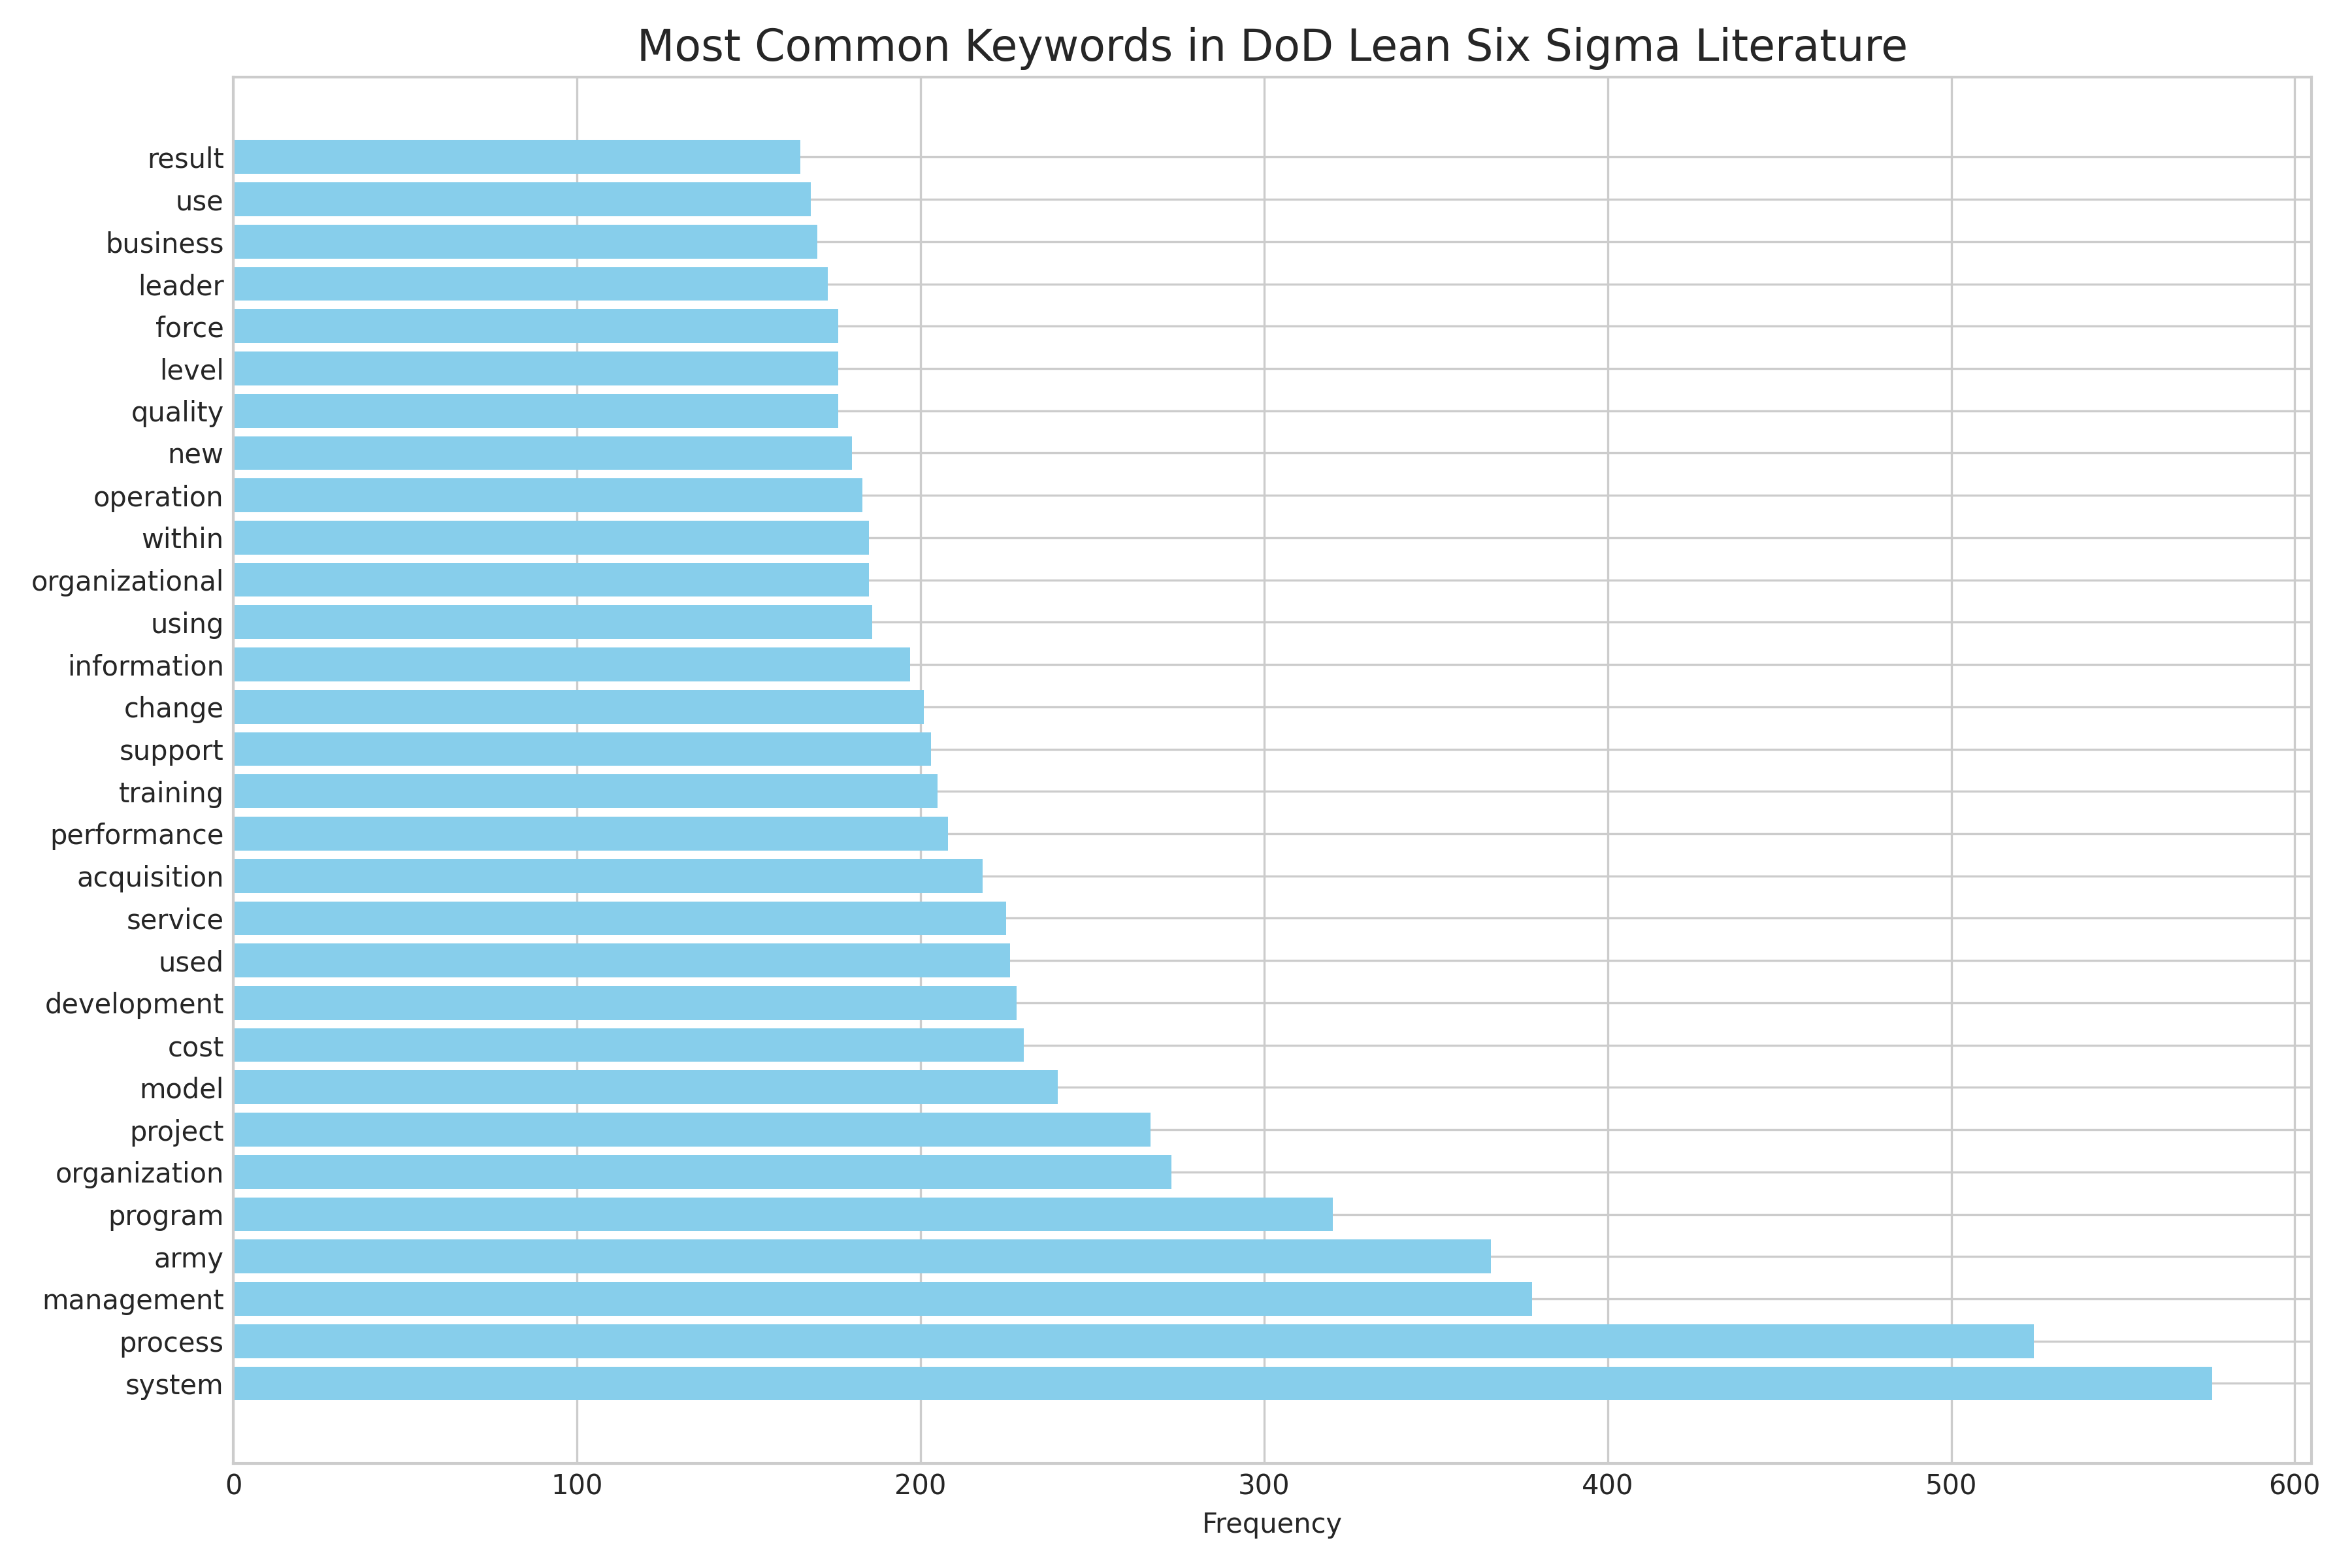
\includegraphics[width=\textwidth,height=0.25\textheight,keepaspectratio]{keyword_frequency}
			\caption{Keyword appearance frequency}
			\label{fig:keyword_freq}
		\end{subfigure}
		\hfill
		\begin{subfigure}[b]{0.32\textwidth}
			\centering
			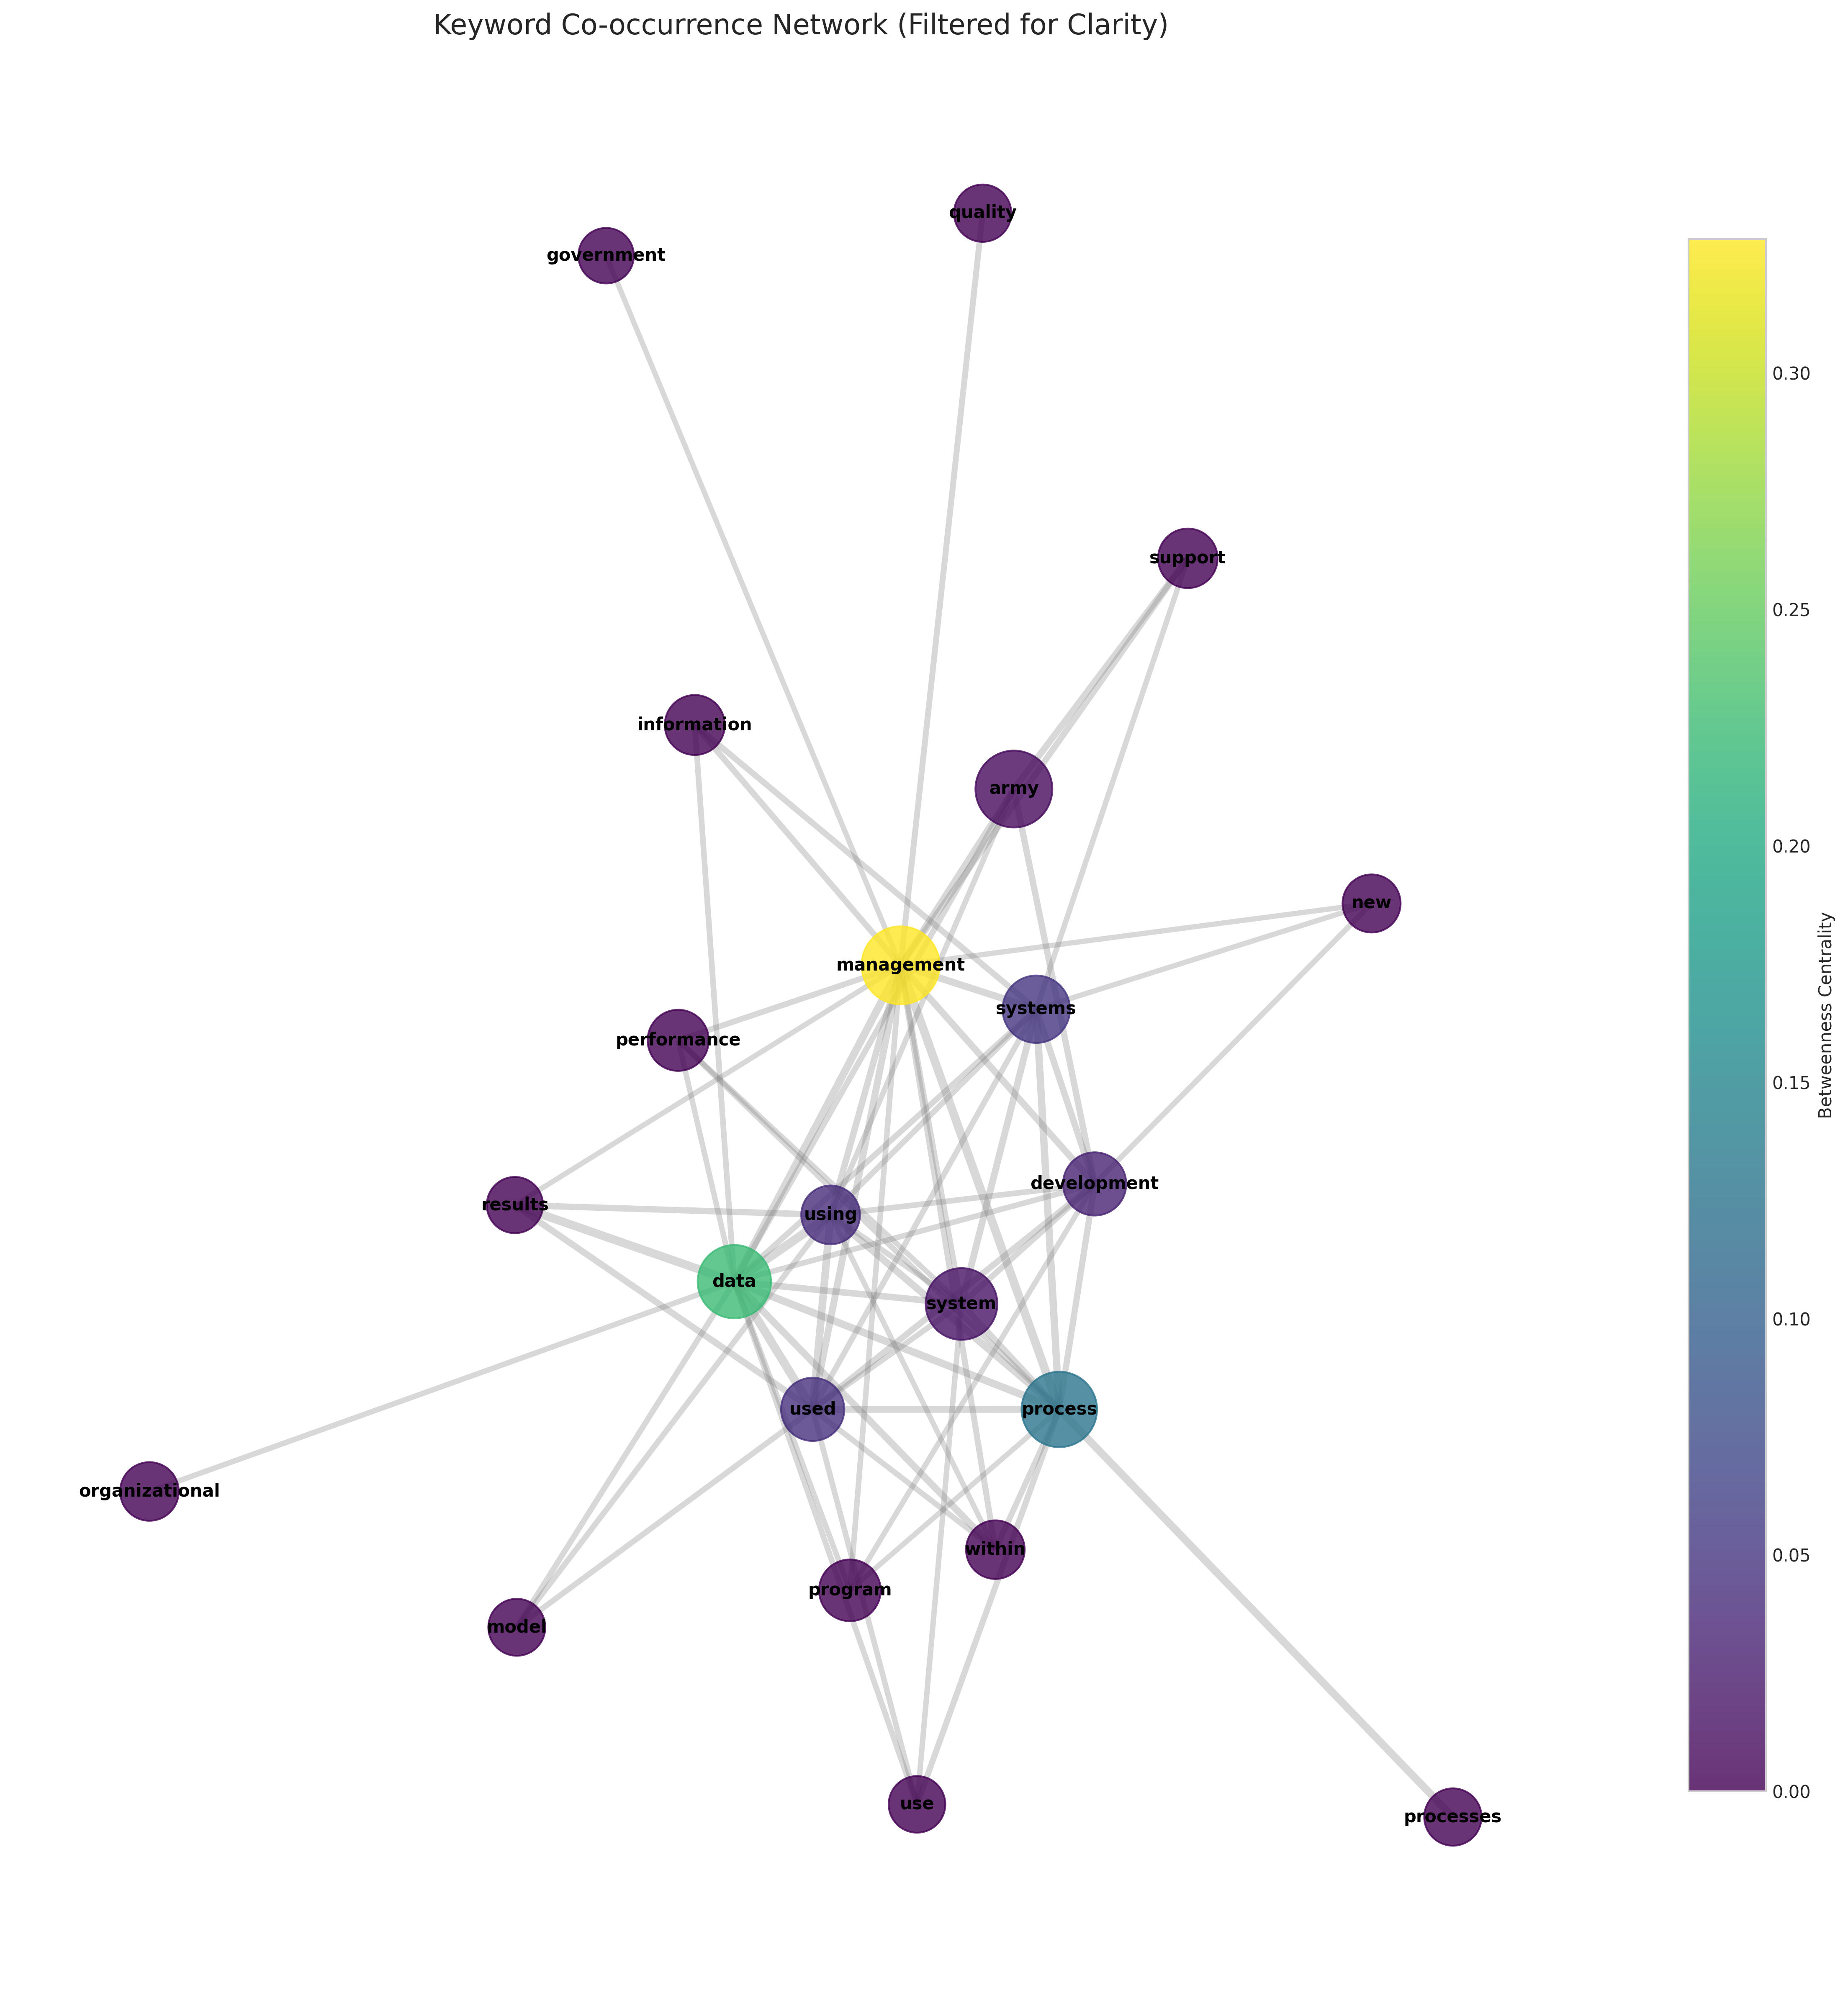
\includegraphics[width=\textwidth,height=0.25\textheight,keepaspectratio]{keyword_network}
			\caption{Keyword co-occurrence network}
			\label{fig:keyword_network}
		\end{subfigure}
		\hfill
		\begin{subfigure}[b]{0.32\textwidth}
			\centering
			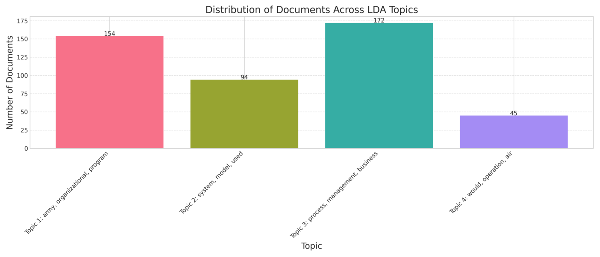
\includegraphics[width=\textwidth,height=0.25\textheight,keepaspectratio]{topic_distribution}
			\caption{Topic distribution from LDA analysis}
			\label{fig:topics}
		\end{subfigure}
		\caption{Keyword analysis and topic modeling results}
		\label{fig:keyword_analysis}
	\end{figure}


	Using all the prior analysis points, the author determined three main themes in the lean six sigma literature: \textit{Management and Leadership, Process Improvement,} and \textit{Continuous Learning}. 
	Using these three themes, a keyword-based categorization algorithm was applied to classify each document according to the most similar theme.

	As visualized in \figref{fig:theme_distribution_bar}, the majority of the papers (54\%) corresponded to the \textit{Management and Leadership} theme, 35.9\% fell into the \textit{Process Improvement} theme, and 9.2\% fell into the \textit{Continuous Learning} theme.
	The distribution of themes over the years is shown in \figref{fig:theme_trends}.


	\begin{figure}[htbp]
		\centering
		\begin{subfigure}[b]{0.48\textwidth}
			\centering
			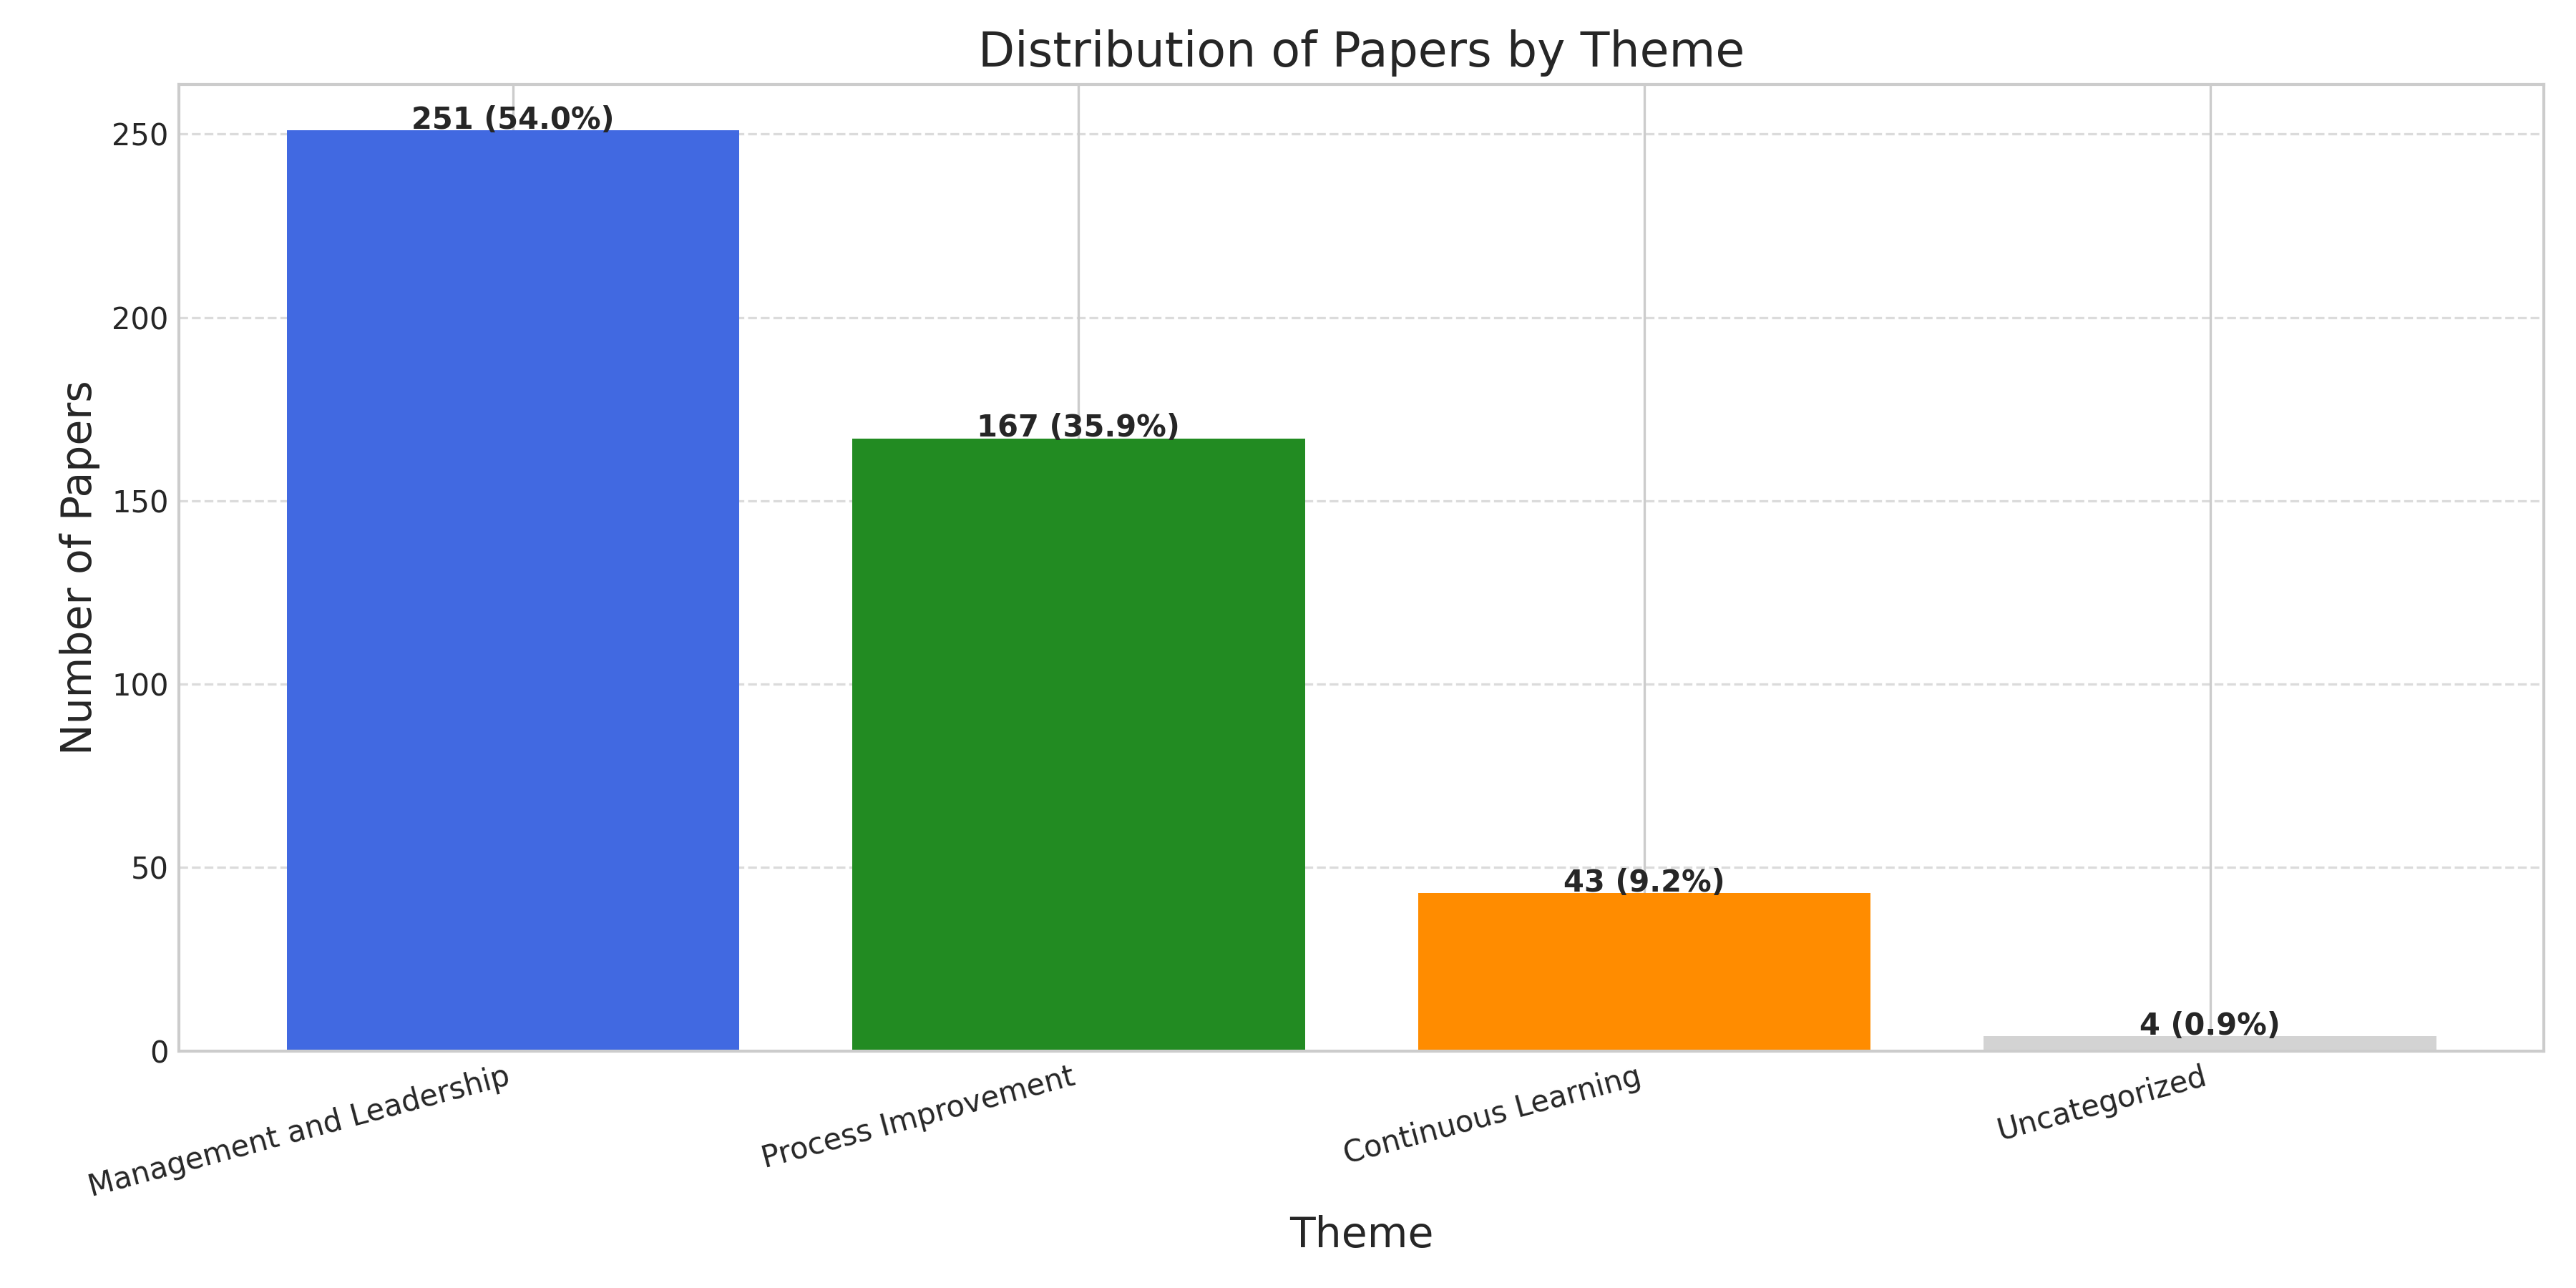
\includegraphics[width=\textwidth,height=0.35\textheight,keepaspectratio]{theme_distribution_bar.png}
			\caption{Distribution of themes in the literature}
			\label{fig:theme_distribution_bar}
		\end{subfigure}
		\hfill
		\begin{subfigure}[b]{0.48\textwidth}
			\centering
			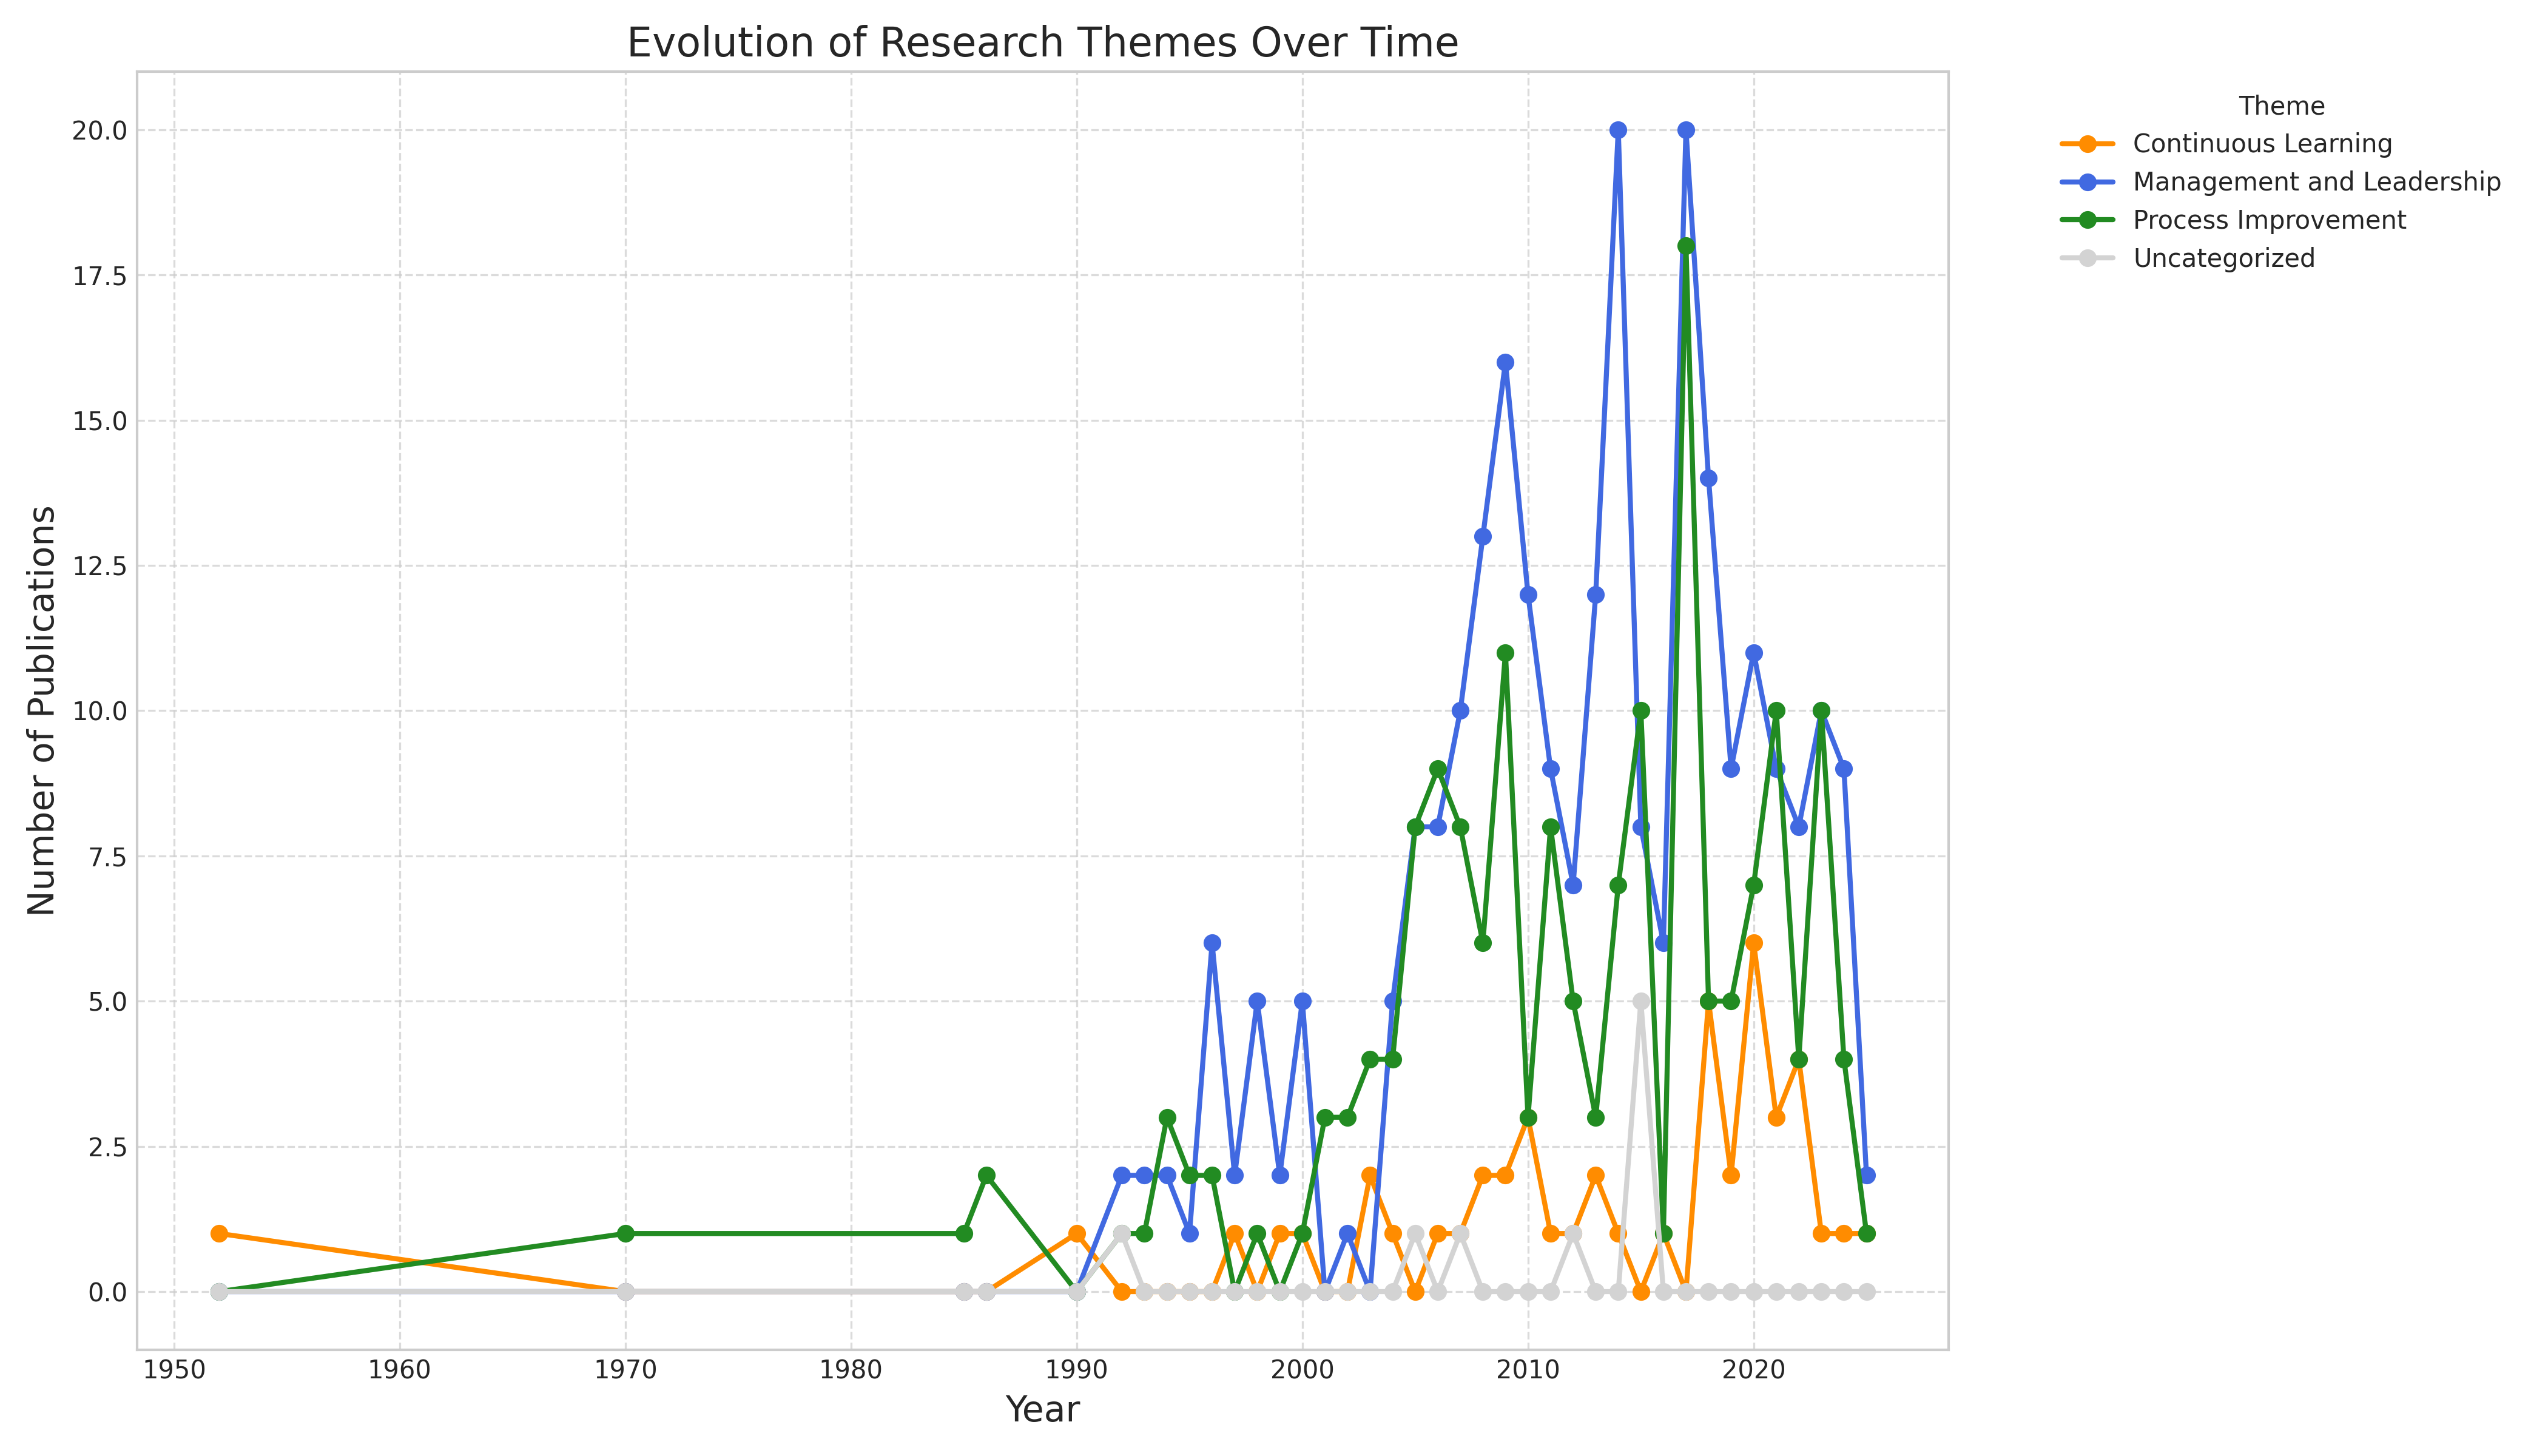
\includegraphics[width=\textwidth,height=0.35\textheight,keepaspectratio]{theme_trends_over_time.png}
			\caption{Theme trends over time}
			\label{fig:theme_trends}
		\end{subfigure}
		\caption{Thematic analysis of lean six sigma literature in DoD contexts}
		\label{fig:theme_analysis}
	\end{figure}



\section{Next Steps and Timeline}
From our scientometric analysis we see that lean six sigma literature relating to the DoD broadly falls into three main themes:
\textit{Management and Leadership}, \textit{Process Improvement} and \textit{Continuous Learning}.
The resulting papers were split according to their theme and recent works in the range of 2020-2025 were selected for further analysis. The works are as follows: 

\begin{itemize}
    \item \textbf{Management and Leadership:} \cite{Turner2024}, \cite{McCants2024}, \cite{Carlstedt2020}, \cite{Malin2020}
    \item \textbf{Process Improvement:} \cite{VanLaar2023}, \cite{Le2023}, \cite{Richmond2023}
    \item \textbf{Continuous Learning:} \cite{FunchesAllen2025}, \cite{Patel2021}
\end{itemize}

In subsequent weeks, the papers will be summarized and analyzed to identify key findings and trends within each theme to provide a comprehensive overview of the current state of lean six sigma literature in the DoD context.

A timeline for this process is given in \figref{fig:timeline}.

% Literature Review Timeline Gantt Chart
\begin{figure}[htbp]
    \centering
    \begin{ganttchart}[
        hgrid,
        vgrid={*1{dotted}},
        x unit=0.8cm,
        y unit title=0.8cm,
        y unit chart=0.8cm,
        title label font=\small\bfseries,
        bar label font=\small,
        milestone label font=\small,
        group left shift=0,
        group right shift=0,
        bar height=0.6,
        bar/.append style={fill=blue!40},
        group/.append style={fill=blue!70},
        milestone/.append style={fill=red, inner sep=2pt}
    ]{11}{19}
        % Month and week numbers
        \gantttitle{Mar}{3}\gantttitle{Apr}{4}\gantttitle{May}{2} \\
        \gantttitlelist{11,...,19}{1} \\
        
        % Tasks
        \ganttbar{Read and analyze: Management and Leadership}{11}{13} \\
        \ganttbar{Read and analyze: Process Improvement}{13}{15} \\
        \ganttbar{Read and analyze: Continuous Improvement}{15}{17} \\
        \ganttbar{Summarize key findings}{17}{18} \\
        \ganttbar{Complete review paper}{18}{19} \\
        \ganttmilestone{Complete presentation slides}{19} \\
    \end{ganttchart}
    \caption{Timeline for literature review by week number}
    \label{fig:timeline}
\end{figure}


\bibliographystyle{IEEEtran}
\nocite{*}
\bibliography{/project/src/ref}

\end{document}